\vspace{3cm}

% \textbf{Àlex Giménez-Romero$^{1}$, Dhafer Ferchichi$^{1}$, Pablo
%     Moreno-Spiegelber$^{1}$, Tomas Sintes$^{1}$,  Manuel A. Matías$^{1}$}

% \vspace{1cm}

% \begin{enumerate}
%     \small
%     \item Instituto de Física Interdisciplinar y Sistemas Complejos, IFISC
%           (CSIC-UIB), Palma de Mallorca 07122, Spain
%     \item Tragsa, Passatge Cala Figuera 6, 07009 Palma de Mallorca, Spain
% \end{enumerate}

% \vspace{1cm}

\textbf{Published as:}

\vspace{0.5cm}

\fullcite{GimenezRomero2024_posi_e}

\newpage
\section{Introduction}

Coastal ecosystems, encompassing seagrasses, mangroves, salt marshes, and coral
reefs, among others, provide invaluable services that contribute to supporting
the livelihoods of coastal communities, impacting the well-being of the
residents \cite{MEA2005,IUCN2008}. Seagrass meadows, in particular, are crucial
for enhancing coastal biodiversity, protecting shorelines from erosion, and
mitigating climate change by sequestering large quantities of carbon
\cite{DuarteNCC2013,Mcleod2011}. However, if these habitats are degraded, they
could leak stored carbon into the atmosphere and further accelerate global
warming \cite{DuarteNCC2013,Macreadie2014}.

In fact, despite the considerable uncertainty surrounding global seagrass
extent values, it is estimated that about one third of seagrass global extent
has been lost since World War II \cite{DuarteNCC2013}. Seagrass declines are
primarily attributed to eutrophication, water quality degradation, habitat
destruction, and climate change, particularly global warming
\cite{Waycott2009}. Furthermore, the
sensitivity of seagrasses to future ocean temperatures under different emission
scenarios poses significant concerns. Models project a decline in the global
suitable habitat for these ecosystems throughout the current century, both
latitudinal and across water depth, with a notable compression of suitable
habitat toward the lower distribution limit imposed by light availability
\cite{Jorda2020}.

In this context, the United Nations (UN) recognized the severity of global
biodiversity loss and degradation of ecosystems and stressed the negative
impact that this situation has on food security, nutrition, access to water,
and the health of the rural poor and people worldwide. Accordingly, the UN
declared the period 2021-2030 as the ``Decade of Ocean Science for Sustainable
Development'' and the ``Decade of Ecosystem Restoration'' \cite{UNdecade2000,
    UNRio}, underscoring the urgency and importance of safeguarding marine
ecosystems, including \textit{Posidonia oceanica} meadows. Achieving these
targets, particularly concerning the preservation and restoration of coastal
ecosystems, requires a rigorous, evidence-based approach to
conservation practice and policy. This entails conducting thorough analyses of
high-quality monitoring data to inform decision-making and validate
intervention strategies.

The comprehensive mapping of several marine habitats,
such as coral reefs, kelp forests, deep-sea vent communities, and seagrass
beds, has been successfully achieved through the use of side-scan sonar systems
\cite{Mumby2002, Mishra2006, LeQuilleuc2022, allen-coral-atlas}. This
methodology has provided valuable insights into the structure and distribution
of these ecosystems and helped to design informed conservation strategies and
management practices. However, the cost and time-intensive nature of these
methods present challenges in deploying continuous monitoring systems for
marine environments. As a result, practical monitoring of biodiversity often
occurs infrequently rather than in real-time, preventing a constant
spatio-temporal evaluation of the status of these ecosystems.

A recently emerging possibility is to combine remote sensing technologies with
available georeferenced habitat data to develop correlative or mechanistic
models that are then capable of monitoring biodiversity at finer temporal
scales. Among various methodologies, Machine Learning (ML) models trained with
multi-spectral satellite imagery data appear to be the most promising
\cite{Zhang2013,Senecal2019,Wicaksono2019,Gudzius2021}. In particular, many
efforts to determine the spatial distribution
of \textit{Posidonia oceanica} from airborne imagery using ML have been
recently made
\cite{Chand2022,Jeon2021,case_study_Aegean_and_ionian_seas,Ariasari2019,comp_study_new_zeeld,MederosBarrera2022,Coffer2020,Marcello2018,Traganos2018c,Poursanidis2019,Duffy2019,Islam2019,Poursanidis2018,Traganos2018b,Traganos2018d,Bakirman2020,Kellaris2019,chowdhury2023ai}.
However, despite the seminal insights of many of these works, they present
numerous limitations that hinder the delivery of functional models suitable for
a real-case deployment, serving merely as potent proof of concept for the
methodologies studied. For instance, many of these studies rely on inadequate
metrics for evaluating model performance in image segmentation problems, such
as accuracy, leading to an overestimation of the model's performance and
neglecting more suitable and demanding metrics like Intersection over Union.
Additionally,
ground truth data predominantly rely on photointerpretation, often with a
limited number of validation points obtained from field data, undermining the
models' robustness. Several studies employ only a single
or few satellite images, limiting the models' generalizability, while there's a
prevalence of simplistic ML methods like Supported Vector Machines
and Random Forests for image segmentation tasks, despite the suitability of
Deep Convolutional Neural Networks (CNN) for such tasks being well-established
\cite{Zeiler2014,Milletari2016}.
Thus, while these studies lay the groundwork for innovative methodologies,
further research is imperative to develop robust and scalable models capable of
meeting the demands of real-world applications in biodiversity monitoring and
management.

To reach this goal, three key considerations need to be addressed.
Firstly, an extensive georeferenced habitat dataset must be employed, acquired
through a meticulous and consistent methodology. This dataset should cover a
broad geographical area and encompass various spatial scales to ensure the
representation of diverse ecological conditions. Secondly, deep learning
models, preferably based on convolutional neural networks (CNNs), should be
trained using a diverse set of satellite images. These images should
incorporate variations in acquisition dates, geographic locations, and the
positions of satellites relative to Earth and the sun. This approach enables
learning under real-world conditions and enhances the robustness of the models.
Lastly, the generalization capability of the models must be evaluated by
testing their predictive performance across regions that are geographically
distinct from the training dataset. These regions should be characterized by
different environmental conditions, ensuring the reliability and applicability
of the models in varied real-world scenarios.

Here, we present a comprehensive framework that addresses these considerations,
providing a robust and reliable model for the classification of
\textit{Posidonia
    oceanica} meadows and related habitats in the Mediterranean Sea using
satellite imagery. We demonstrate the model's generalization capability and
robustness by training only with data from a particular region of our extensive
dataset and evaluating its performance on the other regions. We show that our
model is capable of providing reliable estimates for the distribution of the
considered habitats and accurate measures for their extension area. In
addition, we measure the model's loss of accuracy in its estimates for new
regions, providing a lower bound for model performance. This is a
crucial step to advance in the development of a reliable map of the
distribution of \textit{Posidonia oceanica} meadows in the Mediterranean Sea.
Finally, we train the model with all available data so that the resulting
model can be used to classify posidonia meadows in other regions of the
Mediterranean Sea.

\section{Results}

\subsection{A deep learning framework for automated marine ecosystem
    labelling}

We developed a deep learning framework based on convolutional neural networks
to accurately classify benthic habitats in the Mediterranean Sea using
satellite imagery (\cref{fig:scheme}). We used a comprehensive and extensive
habitat dataset of the Balearic Sea, comprising a 20-year effort of data
acquisition based on side-scan sonar supported by photointerpretation of
high-resolution airborne imagery and in-situ observations (\cref{fig:scheme}a).
The dataset covers  about 2,500 km$^2$ of the coastal habitats of the Balearic
Islands at high spatial resolution and contains 28 different classes,
including the ecologically significant species \textit{Posidonia
    oceanica}, which were aggregated in 4 major ecological groups: Posidonia
oceanica, Other green plants, Rocks \& brown algae, and Sandy bottoms
(\cref{fig:scheme}a,c, Methods \&  \cref{app:satellite_imagery}). This
dataset was combined with satellite imagery of the coastal areas of the
Balearic Islands acquired from PlanetScope \cite{planet2017}, covering around
1200 km$^2$ with different dates and satellite positions (\cref{fig:scheme}b,c,
Methods \& \cref{app:satellite_imagery}).

We trained 40 different deep learning models using 4
different state-of-the-art architectures and 10 different backbones for each
architecture (\cref{fig:scheme}d, Methods \& \cref{app:deep_learning_models}).
Furthermore, we implemented a consensus prediction approach to enhance the
robustness and reliability of model predictions, which involves aggregating the
results from multiple deep learning models to mitigate potential biases
introduced by individual models (Methods). To evaluate the models, we opted for
training only with data from
one island (Mallorca), performing a posterior systematic study of its
performance on the other islands (Menorca, Ibiza, Formentera, and Cabrera).
Thus, the train-test split was roughly 50\%-50\% rather than the traditional
80\%-20\% split, with the test set representing diverse environmental
conditions and benthic habitats formed by slightly different species than
the training set (Methods \& \cref{app:dataset_creation}). This approach
was chosen to simulate real-world scenarios in which one cannot control for
specific environmental conditions, constrained dates for image acquisition, the
position of the satellite with respect to the sun and the earth, or even find
new species not contained in the original training dataset. We thereafter refer
to our test set as ``out-of-sample'' test set and to the model as ``Half
model'' to emphasize this idea.

\begin{figure}[H]
    \centering
    \includegraphics[width=0.87\textwidth]{Figures/scheme.pdf}
    \caption[AI framework for seagrass monitoring from satellite imagery]{(a)
        Spatial distribution of the 4 main ecological benthic habitats
        in the Balearic Sea, present in the whole Mediterranean. The dataset
        provides detailed information at multiple spatial scales up to 3 m
        resolution. (b-d) Scheme of the pipeline to train the CAMELE model.
        Satellite-based surface reflectance data is merged with bathymetric
        estimates to produce the inputs (features) of the model. Habitat data
        obtained with side-scan sonar, photointerpretation and field
        observations were used as ground truth data (labels). These features
        and labels are used to train deep convolutional neural networks to
        perform image segmentation.}
    \label{fig:scheme}
\end{figure}

We performed an extensive evaluation of the models' performance in the
training and out-of-sample test datasets, using a variety of metrics such as
Intersection over Union (IoU), Precision, Recall, F1-score, Kappa and Accuracy
(Methods). Our results show that the best performing framework was to use the
10 models defined by the Linknet architecture together with the consensus
prediction approach (Methods and
\cref{app:architecture_selection,app:out_of_sample}), which hereafter we
refer to as CAMELE (Consensus for Automated Marine Ecosystem Labelling and
Evaluation).

\subsection{A reliable AI-based solution for marine ecosystem monitoring}

CAMELE's performance in both training and out-of-sample test datasets was
highly notable, with a mean IoU score of 88.22\% and a mean F1-score of
93.13\% in the training dataset, compared with a mean IoU score of 61.97\%
and a mean F1-score of 72.77\% in the out-of-sample test dataset
(\cref{fig:model_performance}a and \cref{tab:metrics-train,tab:metrics-test}).
We note that an IoU score greater than 50\% is considered an acceptable
prediction in image segmentation tasks \cite{dai2016instance} (yellow stars in
\cref{fig:model_performance}a). Furthermore, the model outperforms by a large
margin the naive baseline of predicting only the majority class (yellow
diamonds in \cref{fig:model_performance}a). We observe an overlap between the
distribution of the performance metrics in the training and out-of-sample test
datasets, showing that model performance is consistent in both sets
(\cref{fig:model_performance}a). The model was able to segment some images in
the out-of-sample test dataset with notable performance (e.g., 15\% of the
images with an IoU score higher than 80\% and 20\% of the images with an IoU
score higher than 70\%), while only 10\% of the images had an IoU score lower
than 50\% (\cref{fig:model_performance}a and \cref{tab:metrics_img}). This
demonstrates that the model is able to generalize to some extent to new
regions, with different environmental conditions and the presence of some
different benthic habitats.

The decrease in performance in the out-of-sample test dataset can be
attributed to the different environmental conditions, including the
presence of different benthic habitats not included in the test dataset.
However, we observed that a significant part of the pixels categorized by
the ground truth data as Other green plants, Brown algae \& rocks, or Sandy
bottoms were being classified by the model as Posidonia oceanica, substantially
affecting the overall performance of the model
(\cref{app:out_of_sample,fig:confusion_matrix}).
Surprisingly, we found that the distribution of response values for the Other
green plants class in the test dataset is much more similar to the distribution
of response values of the Posidonia oceanica class in the train set
than to its own class
(\cref{app:out_of_sample,fig:similarity_train_test_classes}). Then it is not
surprising that the model classifies all those samples as \textit{Posidonia
    oceanica}. In contrast, the model achieved notable performance in
segmenting the Posidonia oceanica class, with a mean IoU of 77.30\% compared
with the mean IoU of 91.97\% achieved in the training dataset
(\cref{tab:metrics_classes}). At any rate, the model still achieved an overall
notable performance in the out-of-sample test dataset, demonstrating the
generalization capability and robustness of CAMELE and highlighting its
potential for real-world applications in biodiversity monitoring and
management.

CAMELE's performance was further evaluated by comparing the true and predicted
area for each habitat class in each image of the training and out-of-sample
test datasets. The model achieved a notable performance in predicting the area
of the different habitat classes except for the Other green plants class,
as expected from the previous analysis (\cref{fig:model_performance}b,c).
Specifically, the median absolute errors committed in the prediction of the
area of the different habitat classes were 0.98 km$^2$, 0.06 km$^2$, 0.15
km$^2$, and 0.70 km$^2$ in the training dataset, compared with 2.24 km$^2$,
0.26 km$^2$, 0.47 km$^2$, and 1.12 km$^2$ in the out-of-sample test dataset
for the Posidonia oceanica, Other green plants, Rocks \& brown algae,
and Sandy bottoms classes, respectively. However, the relative errors
were 5.61\%, 11.77\%, 6.77\%, and 14.34\% in the training dataset, compared
with 24.92\%, 99.20\%, 28.16\%, and 35.05\% in the out-of-sample test dataset.
Of course, the high relative errors for the Other green plants
class in the out-of-sample test dataset are nonsensical, as the true area of
this class is small, leading to a high relative error. Thus, we observe
that the absolute errors doubled in the out-of-sample test dataset, while the
relative errors increased by a factor of 5. At any rate, the models'
performance in predicting the area of the Posidonia oceanica class was
particularly notable, with relative errors significantly decreasing with
the extent of the area to be predicted, linked to the wider spatial context
available (\cref{fig:model_performance}d). For instance, the median relative
error for true extent areas between 1 and 5 km$^2$ was 30\% (86\% for 95\%
confidence interval) compared with 7\% (86\% for a 95\% confidence interval)
for areas larger than 20 km$^2$.  This finding underscores the importance of
considering the spatial context when predicting the area of benthic habitats,
highlighting the potential of CAMELE to provide reliable estimates for the
distribution and extension of the considered habitats in the Mediterranean Sea.

\begin{figure}[H]
    \centering
    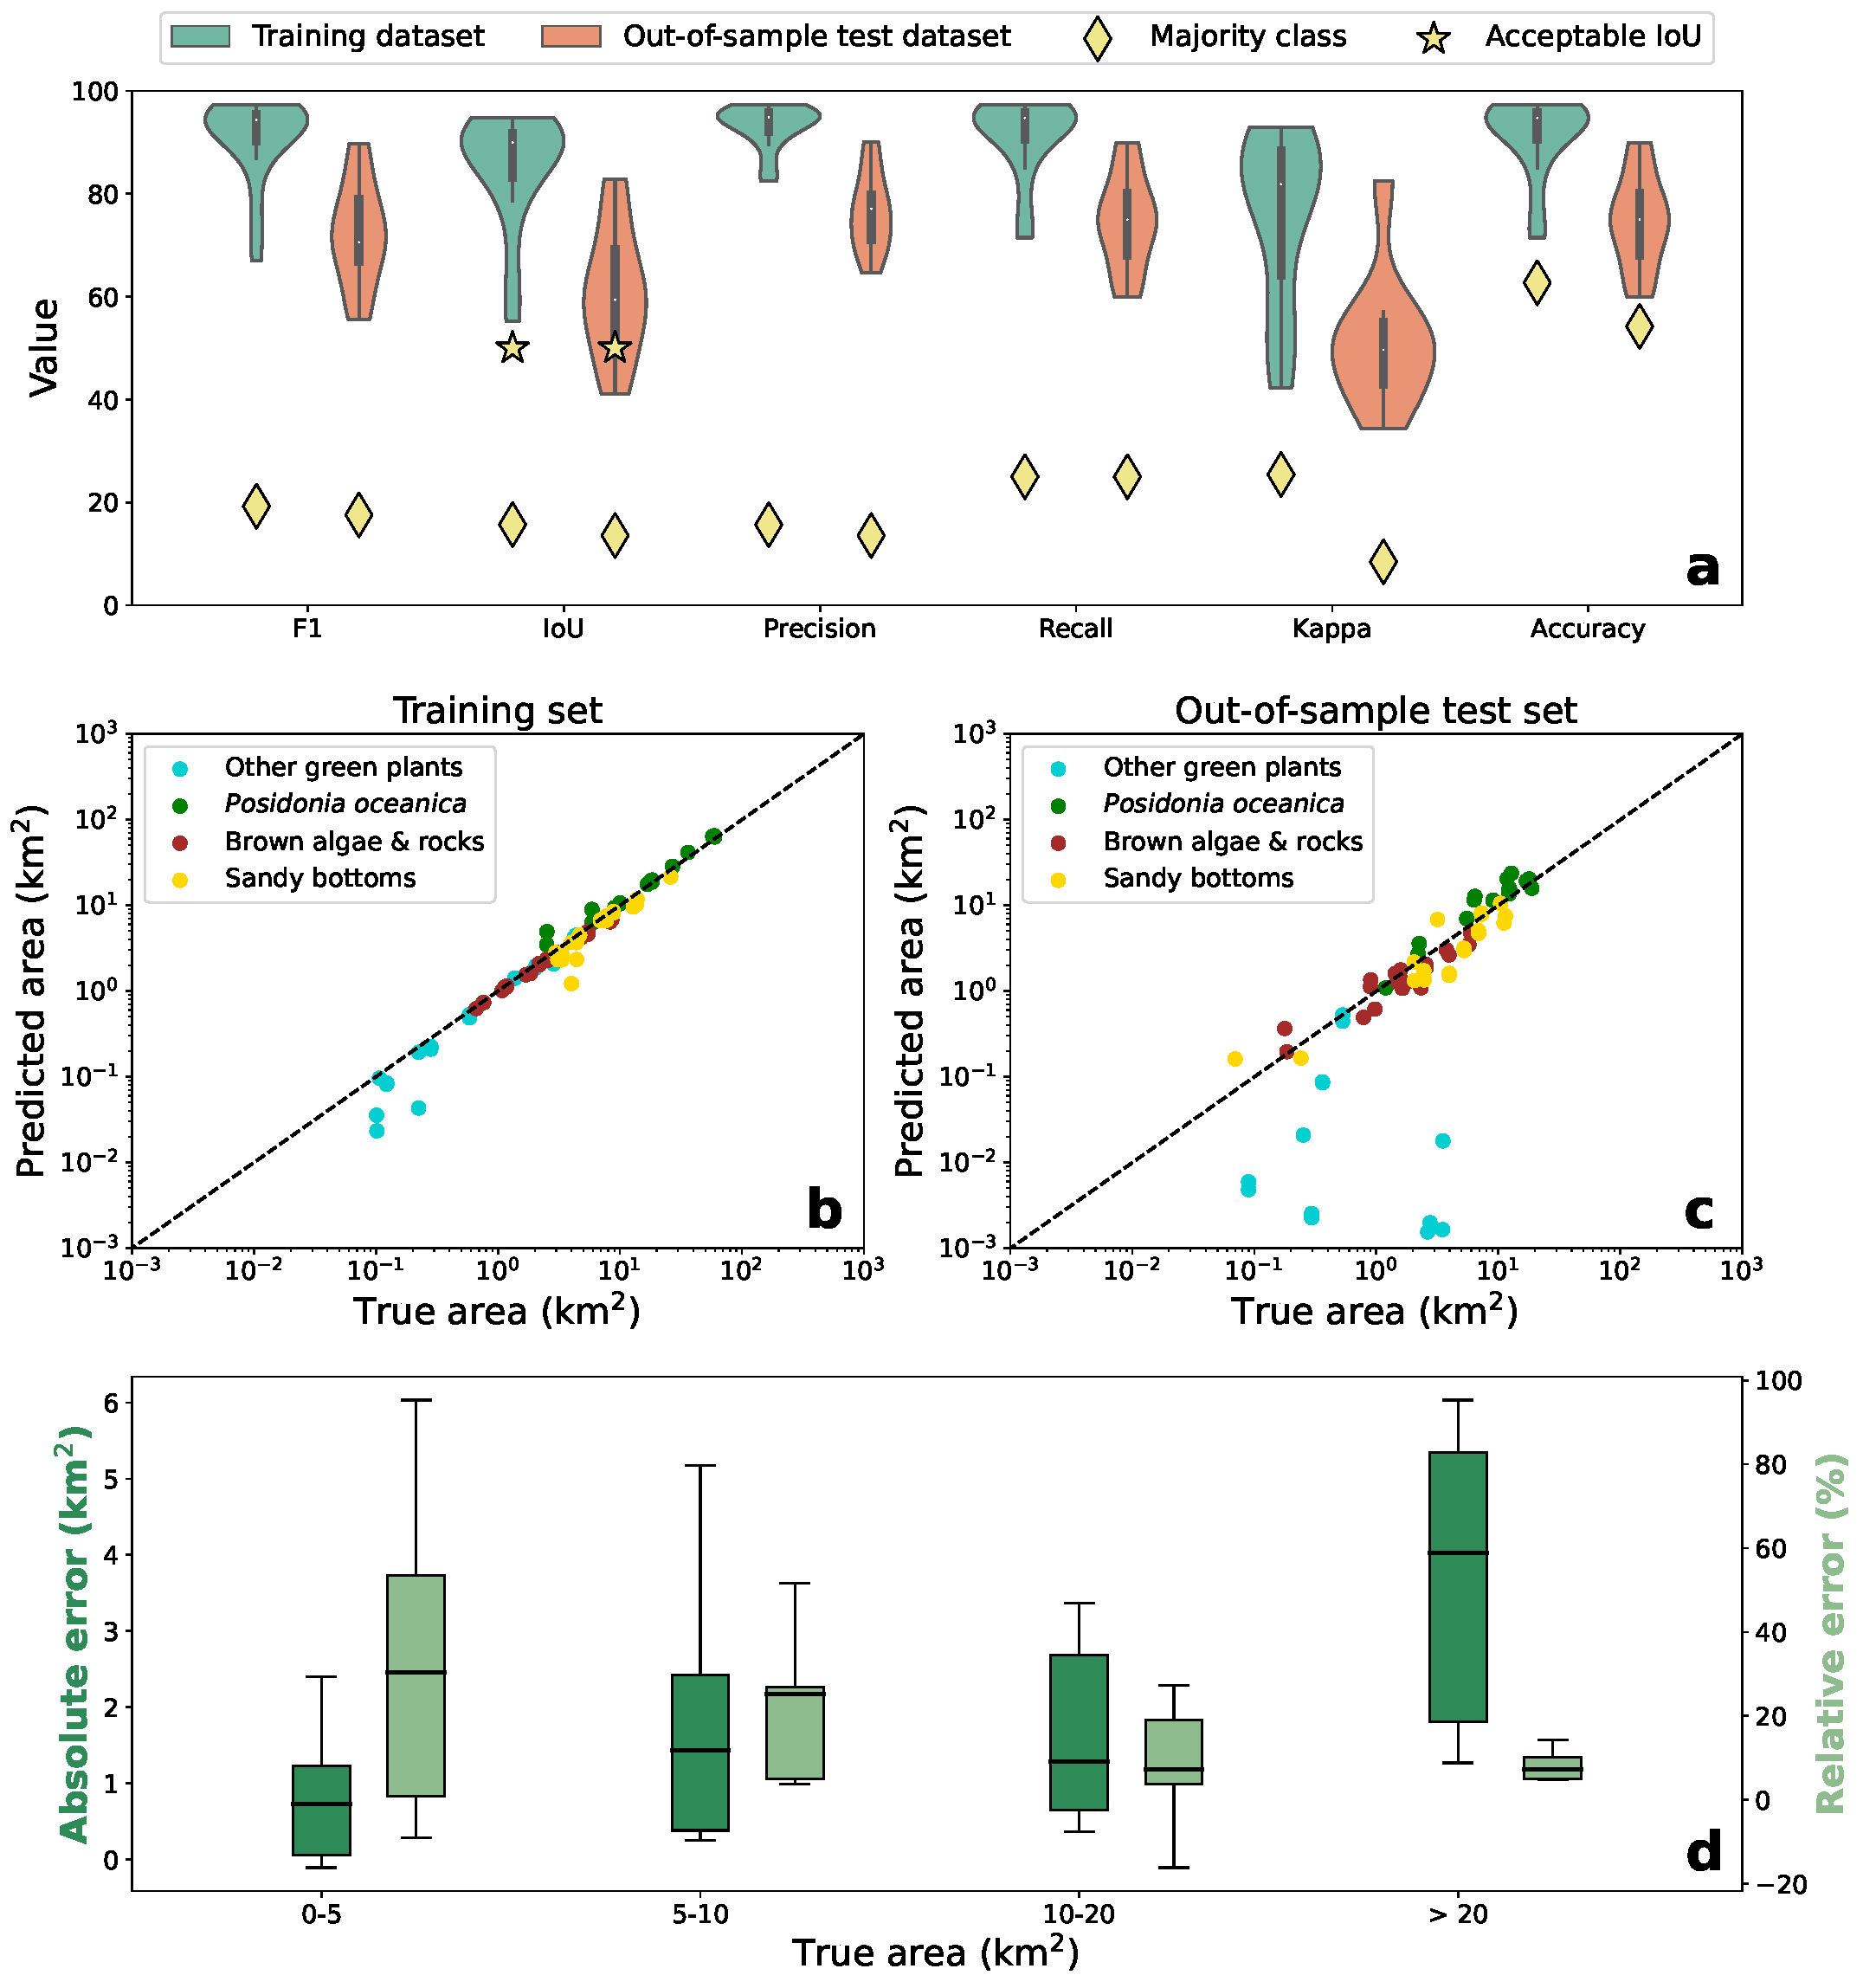
\includegraphics[width=0.95\textwidth]{Figures/Model_performance.pdf}
    \caption[Model performance in train and out-of-sample test datasets]{Model
        performance in train and out-of-sample test datasets. (a)
        Violin plots for F1-score, IoU, Precision, Recall, Kappa and Accuracy
        in both
        training and out-of-sample test datasets. (b-c) True vs predicted area
        for each
        habitat class in the training (b) and out-of-sample test (c) datasets.
        The
        diagonal dashed line indicates perfect prediction. (d) Box plot for the
        absolute
        and relative errors committed in the prediction of \textit{Posidonia
            oceanica}
        area as function of the true area. Relative errors significantly
        decrease with
        the extent of the area to be predicted, linked to the wider spatial
        context
        available.}
    \label{fig:model_performance}
\end{figure}

\begin{figure}[H]
    \centering
    \includegraphics[width=\textwidth]{Figures/Predictions_example.pdf}
    \caption[Example of model predictions for a satellite image in the training
        and out-of-sample test set]{Example of model predictions for a
        satellite
        image in the training
        and out-of-sample test set. (a) Satellite image from Pollença Bay on
        the island of Mallorca, a part of the training set. Image © 2022 Planet
        Labs PBC (b) Ground truth data for the benthic habitats in Pollença
        Bay. (c) Habitat classification from the CAMELE model in Pollença Bay
        (92.78\% IoU). (d) Satellite image from Formentera, part of the
        out-of-sample test set. Image © 2022 Planet Labs PBC (e) Ground truth
        data for the benthic habitats in Formentera. (f) Habitat classification
        from the CAMELE model in Formentera (82.54\% IoU).}
    \label{fig:example_prediction}
\end{figure}

To further illustrate the model's performance, we present an example of model
predictions for a satellite image in the training and out-of-sample test sets
(\cref{fig:example_prediction}). The model accurately classified the different
benthic habitats in both cases with 92.78\% and 82.54\% IoU scores,
respectively, providing reliable estimates for the distribution and extension
of the considered habitats. We note that although there is a 10 point
difference in the IoU score between each prediction, this is almost
unobservable in the visual inspection of the predictions, highlighting the
extreme sensitivity of this metric to small differences.

\subsection{Towards a comprehensive model for the Mediterranean Sea}

Finally, we trained CAMELE with all available data (using 13144 patches for the
actual training and 3286 for the validation set), providing the scientific
community with our final trained models that are freely accessible at
\cite{GimenezRomero_zenodo}. We thereafter refer to this model as the ``final''
model.

We evaluated the performance of the final model in the complete dataset and,
for comparison, also in the previous training and out-of-sample test datasets,
achieving a median IoU score of 95.22\%, 94.73\%, and 96.22\%, respectively
(\cref{tab:my-table}).

\begin{figure}[H]
    \centering
    \includegraphics[width=\textwidth]{Figures/Final_predictions_example.pdf}
    \caption[Example of model predictions for a satellite image in the complete
        dataset]{Example of model predictions for a satellite image in the
        complete
        dataset. The first column shows the ground truth data for the benthic
        habitats, the second column shows the habitat classification from
        CAMELE model trained only with half of the data (from Mallorca island),
        and the third column shows the habitat classification from CAMELE model
        trained with all available data. (a-c) Palma bay, Mallorca. (d-f) Son
        Bou beach, south-east of Menorca. (g-i) Es Còdols, south of Ibiza.
        (j-l) Cala San Vicente, east of Ibiza.}
    \label{fig:model_performance_complete}
\end{figure}

Notably, the model's segmented all the images in the complete dataset with an
IoU score higher than 90\%, with a mean, median, and maximum IoU score of
94.64\% 95.22\%, and 98.5\%, respectively (\cref{tab:metrics_img_final}).
Finally, we assessed the model's robustness by predicting on a new set of
images
from the Balearic Islands in 2023, not used in the training or out-of-sample
test datasets. The model achieved a remarkable mean IoU score of 80\% in this
new dataset (\cref{tab:metrics_img_final_2023,tab:avg_performance_2023}).

\begin{table}[H]
    \centering
    \caption[Final model performance]{\textbf{Final model performance.}
        Performance (IoU score) of the final model in the complete dataset
        and
        comparison with the previous model performance and previous data splits
        conforming the training and out-of-sample (OOS) test datasets.}
    \label{tab:my-table}
    \begin{tabular}{lccc}
        \hline
                                       & \textbf{Train (Half Model)}
                                       &
        \textbf{OOS test (Half Model)} &
        \textbf{Complete
            dataset}
        \\
        \hline
        \textbf{Half model}            & 88.22
                                       & 61.97                       &
        79.21
        \\
        \textbf{Final model}           & 94.73
                                       & 96.22                       &
        95.22
        \\\hline
    \end{tabular}
\end{table}

In \cref{fig:model_performance_complete}, we present some examples of model
predictions in different regions of the Balearic Islands, showing the
ground-truth data for the benthic habitats, the habitat classification from
the CAMELE model trained only with half of the data (from Mallorca island), and
the habitat classification from the CAMELE model trained with all available
data. We observe that the main differences between the predictions of the two
models occur in the areas with more complex habitat distribution. In these
areas, the model trained with all available data is able to capture the
complexity of the habitat distribution more accurately, providing a more
detailed and reliable classification of the benthic habitats. In any case, the
model trained only with data from Mallorca still provides a notable performance
in segmenting the \textit{Posidonia oceanica} meadows from the other islands,
which in the end is the most important habitat to be monitored. A web-based
application for interactively visualizing all model predictions, together
with the ground truth data, is available at \cite{Webpage_camele}.

\section{Discussion}

The present study represents a significant advancement in the field of marine
habitat
monitoring, leveraging the synergistic combination of remote sensing data and
machine learning algorithms to address critical challenges in biodiversity
conservation. Unlike previous studies, we have developed a comprehensive
framework for classifying \textit{Posidonia oceanica} meadows from
multi-spectral satellite imagery based on deep convolutional neural networks,
which in the last years have been shown to be highly effective in image
segmentation tasks. This approach takes advantage of both the rich spectral
and spatial information provided by satellite imagery and the capacity of deep
learning models to learn complex patterns and relationships in the data. In
addition, our analyses do not rely on a single or few satellite images but
rather on a comprehensive dataset of satellite images, covering a wide
geographical area and various spatial scales, to ensure representation of
diverse ecological conditions. This approach is crucial for training models
under real-world conditions and enhancing their robustness and generalization
capability. Indeed, here we make a substantial effort to evaluate the model's
generalization capability by testing its predictive performance across regions
geographically distinct from the training dataset, characterized by different
environmental conditions, to ensure its reliability and applicability in varied
scenarios. Of course, this would not have been possible without the extensive
and detailed georeferenced habitat dataset used in this study.

% \subsection*{Model Generalization and Transferability}
One of the key findings of our study is the remarkable generalization ability
of our deep learning model across different regions of the Balearic Islands.
Despite being trained exclusively on data from a specific area, the model
demonstrated the capacity to provide reliable estimates of \textit{Posidonia
    oceanica} distribution in other islands, where environmental conditions and
benthic habitats vary. This highlights the robustness of our approach and its
potential for broader applicability in marine habitat monitoring. The ability
of the model to generalize across regions is crucial for its practical utility
in conservation efforts beyond the training domain. By accurately classifying
marine habitats in unseen environments, our model showcases its capacity for
real-world application, particularly in scenarios where comprehensive training
data may be limited. Furthermore, the provided metrics, including median
absolute and relative errors in \textit{Posidonia
    oceanica} area prediction, offer valuable insights into the model's
performance and potential limitations. By quantifying prediction errors and
their relationship to true area estimates, we establish a foundational
understanding of the model's accuracy and reliability, enabling more informed
decision-making in habitat monitoring and conservation efforts.

% \subsection*{Integration of Remote Sensing and Machine Learning for Biodiversity Monitoring}
The combination of remote sensing and Machine Learning holds promise for
revolutionizing biodiversity monitoring, offering unprecedented opportunities
for conservationists, policymakers, and researchers to make informed decisions
and address pressing environmental challenges. With its ability to provide
near-real-time data on ecosystem dynamics, our approach offers a cost-efficient
and scalable solution for continuously assessing biodiversity distribution in
the Mediterranean Sea, allowing to identify habitat degradation and monitor
ecosystem resilience in the face of environmental change. This is particularly
crucial in the context of the ongoing climate crisis, where the ability to
rapidly detect and respond to habitat loss and degradation is essential for
preserving marine biodiversity and ecosystem services. Thus, our model
represents a powerful tool in the conservation toolbox, enabling timely
interventions supporting the sustainable management of coastal ecosystems and
the preservation of biodiversity for future generations.

% \subsection*{Challenges and Limitations}
Despite the notable advancements and potential of our study, several challenges
and limitations remain to be addressed. Firstly, the reliance on satellite
imagery for habitat classification presents inherent limitations, including
cloud cover, atmospheric interference, and limited spatial and spectral
resolution, which may impact the accuracy and detail of habitat classification,
especially in complex coastal environments. Additionally, the availability and
quality of training data pose challenges, as incomplete or biased datasets can
impact model performance and generalization capabilities. Moreover, our
analysis focused on 4 major aggregated ecological groups, including
\textit{Posidonia oceanica} habitats, neglecting other important benthic
species and ecosystems that contribute to overall marine biodiversity.
Furthermore, while our models exhibit robustness in cross-regional
generalization within the Balearic Islands, their applicability to other
geographical regions with distinct environmental conditions remains untested.
Thus, it may exhibit limitations in delineating finer-scale habitat features in
regions with distinct ecological characteristics. Addressing these limitations
through continued data collection, model refinement, and validation efforts
will be crucial for advancing the reliability and applicability of remote
sensing-based approaches in marine habitat monitoring and conservation.

% \subsection*{Future Directions}
Looking ahead, several avenues for future research and practical applications
emerge from our study. Firstly, continued efforts to expand and refine training
datasets, incorporating data from diverse geographic regions and ecosystem
types, will further enhance the accuracy and generalization capabilities of
machine learning models for marine habitat monitoring. Additionally, ongoing
advancements in remote sensing technology, including the development of higher
spatial and spectral resolution sensors, hold promise for improving habitat
classification accuracy and detail. Integration with emerging techniques such
as drone-based imaging and LiDAR further expands the scope and resolution of
habitat monitoring efforts, enabling finer-scale analysis and management.
Moreover, the development of user-friendly tools and platforms for data
visualization and decision support facilitates the translation of scientific
findings into actionable conservation strategies. By empowering stakeholders
with accessible and interpretable information, we can foster greater engagement
and collaboration in marine conservation initiatives, ultimately contributing
to the sustainable management of coastal ecosystems and the preservation of
biodiversity.

In conclusion, our study represents a significant step forward in the field of
marine habitat monitoring, showcasing the transformative potential of remote
sensing and machine learning technologies. By advancing our understanding of
ecosystem dynamics and supporting evidence-based conservation practices, our
work contributes to the broader mission of safeguarding marine biodiversity for
future generations.

\section{Methods}

\subsection{Satellite data}

Satellite imagery was obtained from Planet under the Education and Research
Program, which provides limited, non-commercial access to PlanetScope and
RapidEye imagery \cite{planet2017}. In particular, we acquired PlanetScope
images obtained through the Super Dove (PSB.SD) instrument, which consists of
Coastal Blue, Blue, Green I, Green, Yellow, Red, Red Edge and NIR and operates
from 2020. Surface Reflectance (SR) products were selected to ensure
consistency across localized atmospheric conditions, minimizing uncertainty in
spectral response across time and location. SR is derived from the standard
Analytic Product (Radiance) and is processed to top-of-atmosphere reflectance
and then atmospherically corrected to bottom-of-atmosphere reflectance.

We obtained a total of 60 satellite images along the coast of the Balearic
Islands, covering up to 1200 km$^2$ of surface area for the years 2020 to 2023
(\cref{app:satellite_imagery,fig:images-dataset}). The images were
acquired for days with clear sky conditions comprised between June and
September, as these are the months in which the biomass of seagrass and algae
is more abundant. No other filters were applied to the images, as we aimed to
train the model in real-case scenarios in which one cannot control for specific
environmental conditions, constrained dates for image acquisition, the position
of the satellite with respect to the sun and the earth, etc. Thus, we obtained
images with different conditions
(\cref{app:satellite_imagery,tab:metadata_satellite_images}).

\subsection{Habitat data}

We used georeferenced habitat data from the government of the Balearic
Islands, corresponding to the outcome of different European and national
projects comprising a $\sim~20$-year effort of data acquisition covering a
total of 2,500 km$^2$ \cite{cartografia,ValleVillalonga2023}. The first
project started around the year 2000, and there has been a major recent update
around 2018. The data consist of 28 different habitat classes following the
nomenclature and coding of the Standard List of Marine Habitats of Spain
(LPHME), obtained from side scan sonar, photointerpretation of airborne
imagery, and in-situ observations. We aggregated the different habitat classes
into 4 major ecological groups present in the whole Mediterranean Sea. The
aggregation was based on feature similarity and ecological function, resulting
in the following classes: Posidonia oceanica, green algae, brown algae \&
rocks, and sandy bottoms
(\cref{app:satellite_imagery,tab:ecological_categories}).

\cref{fig:scheme}a shows the spatial distribution of the considered ecological
groups in the Balearic Sea. This comprehensive dataset provides detailed
information at multiple spatial scales, offering a valuable insight into the
intricate spatial patterns of the different habitat classes across the region.
The detailed information captured by the high-resolution data contributes
significantly to the reliability of our model and the precision of our
predictions, particularly vital in the context of habitat
conservation for \textit{Posidonia oceanica} meadows.

\subsection{Bathymetric data}

Bathymetric data was obtained from the European Marine Observation and Data
Network (EMODNET) \cite{emodnet}. EMODnet-Bathymetry provides a service for
viewing and downloading a harmonised Digital Terrain Model (DTM) for the
European sea regions. The data consist of GeoTIFF layers with $\sim100$ m pixel
resolution of mean depth values.

\subsection{Dataset creation}

Satellite images were processed together with habitat and bathymetric data to
construct the final training and testing datasets. The NIR band, which is
strongly attenuated by water, was used to mask out pixels corresponding to land
using a simple clustering algorithm (i.e., K-means) and subsequently
substituted
for bathymetric data. The resulting processed
satellite images comprise the primary source for the input data of our model.
The ground truth (or label) dataset consists of raster files analogous to the
satellite image with single-band values representing the benthic class
corresponding to each pixel. To construct it, all pixels of each processed
satellite image were associated to a given benthic class using the aggregated
habitat data. Pixels for which a class was not available were masked out in
both the processed satellite image and label data. Similarly, pixels that were
already masked in the satellite image were masked in the label image. Finally,
patches measuring 256 x 256 pixels ($\sim 750\,m \cross 750\,m$) were extracted
from each satellite and label image for the years 2020 to 2022 (keeping the
year 2023 as a final test), resulting in a final dataset comprising up to
16,430 patches.

Despite train-test data split usually follows an 80\%-20\% ratio, training was
conducted exclusively with data from Mallorca (8488
patches, of which 1698 were allocated for validation) and tested with the
remaining data from Menorca, Ibiza, Formentera, and Cabrera islands (7942
patches), following a roughly 50\%-50\% train-test split. Furthermore, our
test set represented diverse environmental conditions and even benthic habitats
formed by slightly different species than the training set, thereby simulating
real-world scenarios that the model may encounter in operational settings. By
testing the model on data from regions beyond its training domain, we aimed to
assess its generalization ability and robustness. Specifically, we sought to
determine whether the model could accurately classify marine habitats and
benthic features in unseen environments, probably slightly different from the
ones at training, thereby demonstrating its capacity for real-world
application. We thereafter refer to our test set as ``out-of-sample'' test set,
to emphasize this idea. All images from 2023 were kept for a final test to
analyze model robustness once it is trained with data from all regions in the
years 2020 to 2022.

\subsection{Deep learning models}

We trained different state-of-the-art deep learning models for semantic image
segmentation, such as UNET \cite{Ronneberger2015}, Linknet
\cite{Chaurasia2017}, FPN \cite{Lin2017}, and PSPNet \cite{Zhao2017}. Each
architecture is formed by repeating convolutional blocks, which are usually
referred to as the ``backbone'' of the model. We tested 10 different backbone
models for each architecture, leading to the training and evaluation of 40 deep
learning models, which represents an unprecedented effort in the field. We
used the segmentation-models Python library \cite{segmentation_models} to
define and train all models.

\subsection{Model training}

Before training, the input data was standardized using the mean and variance of
the training data,
\begin{equation}
    z=\frac{X-\mu}{\sigma} \ .
\end{equation}
This standard scaling procedure ensures that all input features have a
consistent scale, preventing the dominance of certain features during the
training process. It is crucial to note that the same standard scaling
procedure must be applied during predictions, using the mean and standard
deviation computed from the training set. This consistency ensures that the
model interprets new data comparably to the training data.

Additionally, for the categorical nature of the output, labels were one-hot
encoded. This encoding converts categorical labels into binary vectors, where
each class is represented by a unique binary value, facilitating the model's
interpretation of the multi-class classification task.

In terms of loss function selection, we opted for dice loss due to its
effectiveness in handling imbalanced datasets, a common characteristic in tasks
involving semantic segmentation \cite{rahman2016optimizing}. Dice loss, also
known as the Sørensen–Dice coefficient \cite{sorensen1948method,
    dice1945measures}, measures the similarity between predicted and ground
truth data by computing the intersection over the union of the two. To further
account for class imbalance, we applied loss weights inversely proportional to
the proportion of examples of each class. The learning rate was set to 0.001 to
ensure a smoother training process.

The models were trained in a computing cluster, using 10 cores and a maximum of
400 GB of RAM for each model. The training process was performed for 1000
epochs with a batch size of 32. The total training time was approximately 1
month for the 40 initial models using the data from the island of Mallorca and
about 3 months for the 10 final models using all available data.

\subsection{Performance metrics}

The performance of our trained models was primarily evaluated by the
Intersection over Union (IoU) score (\cref{eq:IoU}), which evaluates the
spatial overlap between the predicted image and the ground truth, as this is a
suitable metric for image segmentation problems \cite{rahman2016optimizing}.
Additionally, we considered other metrics such as accuracy
(\cref{eq:accuracy}), precision (\cref{eq:precision}), recall
(\cref{eq:recall}), F-1 score (\cref{eq:f1_score}), and Cohen's Kappa
(\cref{eq:kappa}) to perform a comprehensive evaluation of the model. Accuracy
gauges the overall correctness of predictions, precision measures the accuracy
of positive predictions, recall assesses the model's ability to capture all
positive instances, and the F-1 score provides a balanced assessment of
precision and recall. For a binary classification problem, the metrics can be
defined from the confusion matrix, where TP, TN, FP, and FN represent true
positives, true negatives, false positives, and false negatives, respectively,
and $N$ is the total number of pixels in the image.

\begin{equation}\label{eq:accuracy}
    \text{Accuracy} = \frac{TP + TN}{N}
\end{equation}

\begin{equation}\label{eq:precision}
    \text{Precision} = \frac{TP}{TP + FP}
\end{equation}

\begin{equation}\label{eq:recall}
    \text{Recall} = \frac{TP}{TP + FN}
\end{equation}

\begin{equation}\label{eq:f1_score}
    \text{F1 Score} = \frac{2\times TP}{2\times TP + FN + FP}
\end{equation}

\begin{equation}\label{eq:kappa}
    \kappa=\frac{2\left(TP\times TN - FP\times FN\right)}{(TP + FN)(FN + TN) +
        (TP + FP)(FP
        + TN)}
\end{equation}

\begin{equation}\label{eq:IoU}
    \text{IoU} = \frac{\abs{P\cap L}}{\abs{P\cup L}}=\frac{TP}{TP + FP + FN}
\end{equation}

These metrics collectively offer a holistic understanding of the model's
effectiveness in classifying benthic habitats. See Supplementary Information
for further details.

\subsection{Consensus prediction}

We implemented a consensus prediction approach to enhance the robustness and
reliability of model predictions. The consensus prediction involves aggregating
the results from multiple deep learning models, each trained with different
architectures and backbones. By combining predictions from diverse models, we
aim to mitigate potential biases introduced by individual models and enhance
the overall accuracy and generalization capabilities.

For each input patch, predictions from all trained models were collected, and a
voting mechanism was employed to determine the final consensus prediction.
Specifically, the class label with the highest frequency across all model
predictions was assigned to each pixel. This ensemble-based strategy
leverages the diversity of information captured by different models, leading to
a more robust and reliable classification outcome.

\subsection{Model selection}

To filter among the 4 different architectures, we evaluated the models'
performance in the training dataset. Despite all models achieved high IoU
scores ($> 0.8$), Linknet and UNET architectures were the best performing
models with a mean IoU of 90.98\% and 90.90\%, respectively
(\cref{tab:metrics-architectures}). Because Linknet architecture has less
trainable parameters than UNET, being more efficient in terms of computational
resources and less prone to overfitting, we selected it as the final
architecture to build CAMELE, finally consisting of 10 different models
(\cref{app:architecture_selection}).

We then evaluated the performance of each of the 10 models and the consensus
prediction approach in the training and out-of-sample test datasets
(\cref{app:out_of_sample}). All models achieved high performance, with a median
IoU of 88.12\% and F1-score of 93.16\% in the training dataset
(\cref{tab:metrics-train}), while the models' performance in the out-of-sample
test dataset was significantly reduced, with a median IoU of 60.73\% and
F1-score of 71.87\% (\cref{tab:metrics-test}). When analyzing the performance
of the models individually, we observed the emergence of ``specialists'', which
performed significantly better than the rest of the models in segmenting
specific classes. This finding underscores the importance of the consensus
prediction approach, which leverages the diversity of information captured by
different models. The consensus prediction approach significantly improved the
models' performance in the out-of-sample test dataset, with an IoU score of
61.97\% and a F1-score of 72.77\% (\cref{tab:metrics-test}), highlighting the
effectiveness of the ensemble-based strategy in mitigating potential biases
introduced by individual models and enhancing the overall accuracy and
generalization capabilities of CAMELE. Thus, the consensus prediction approach
was selected as the final model for CAMELE.